\documentclass[11pt,reqno]{amsart}
%%% WARNING: Do NOT change the page size, fonts, or margins!  Penalties will apply.


\usepackage{graphicx}
\usepackage{amssymb,amsmath,amsthm, amsmath, amsthm, amscd, amsfonts, amssymb, graphicx, color}
\usepackage{placeins} %enables \FloatBarrier, that prevents floats from going below it.


%%% WARNING: Do NOT change the page size, fonts, or margins!  Penalties will apply.
%%% WARNING: Do NOT change the page size, fonts, or margins!  Penalties will apply.

\newtheorem*{remark}{Remark}

\begin{document}

\title{The Simeoni Model for Tumor Growth}
\author{Sophie Carter, Morgan Nielsen, Michelle Wang, Sarah Winters}
\date{December 7, 2023}


\maketitle

\begin{abstract}
The Simeoni Model is a system of ordinary differential equations that represents tumor growth as it receives different treatments. After researching the constants, variables, and functions used in this model, we created graphs to see how changing the parameters affected the model and what it implied about tumor growth. We conclude that this model successfully represents immunotherapeutic and chemotherapeutic treatment on tumor cells, and we are curious about how the different constants are related to the various cancer treatments. 
\end{abstract}

%% First Section
\section{Background/Motivation}
As a team, our search for a suitable situation or phenomenon to model encountered some obstacles. Initially, many concepts we considered were better suited for a Partial Differential Equation (PDE) rather than an Ordinary Differential Equation (ODE), which we aimed to avoid based on advice from our professor. Additionally, we sought a topic with a significant impact on people's lives. This led us to focus on analyzing the Simeoni Model (1.1), specifically its application in modeling cancerous tumor growth within the body \cite{Koziol_Falls_Schnitzer_2020}.

Cancer is a complex group of diseases characterized by the uncontrolled division and growth of abnormal cells, which can infiltrate and destroy normal tissues within the body. Tumor growth, a hallmark of cancer, poses a critical threat as it can lead to the disruption of essential physiological processes by cutting off the oxygen and nutrient supply to surrounding tissues \cite{Cancer_Research_2023}. As cancer progresses, it often metastasizes, spreading to other parts of the body and compounding the challenges of treatment. The profound impact of cancer on individuals' lives, coupled with the urgent global quest for improved solutions and treatments, underscores the importance of studying and modeling tumor growth.

Our motivation for selecting the Simeoni Model as the focus of our research stems from its application in addressing the intricate dynamics of cancerous tumor growth within the body. By delving into this modeling framework, we aim to contribute to existing research efforts seeking to better understand solutions and treatments for cancer. The Simeoni Model provides a valuable platform for simulating and understanding the intricate processes involved in tumor development. Analyzing and modifying this model can offer insights into the underlying mechanisms of cancer progression, potentially leading to more effective strategies for intervention and treatment. Ultimately, our research endeavors aspires to contribute to the broader goal of preventing the devastating consequences of uncontrolled tumor growth and, in turn, improving the prognosis and quality of life for individuals facing cancer diagnoses.


%% Second Section 
\section{Modeling}
While the Simeoni model and the SIR model represent different phenomena, they share similarities in certain aspects, such as their mathematical structures and underlying conceptual framework, which illustrate the relevance of our project to our classwork. In particular, both models utilize a system of differential equations to describe the dynamics of populations. In both cases, a portion of the population undergoes a transition, such as infection or initialization of cell death, in one equation, and this affected population is then incorporated into the subsequent equation. This sequential flow of individual entities from one compartment to another reflects the progression of the affected population through distinct stages.

\begin{equation}\label{eq:1.1}
\begin{aligned}
    \frac{dZ_1}{dt} &= TGF(t) - k_1c(t)Z_1(t), \\
    \frac{dZ_2}{dt} &= k_1c(t)Z_1(t) - k_2Z_2(t), \\ 
    \frac{dZ_3}{dt} &= k_2Z_2(t) - k_2Z_3(t), \\
    \frac{dZ_4}{dt} &= k_2Z_3(t) - k_2Z_4(t)
\end{aligned}
\tag*{(1.1)}
\end{equation}
\hspace{2em}

\hspace{2em}

\begin{equation} \label{eq:1.2}
\begin{aligned}
    TGF(t) &= \frac{\lambda_0Z_1(t)}{[1 + (\frac{\lambda_0}{\lambda_1}V(t))^\psi]^\frac{1}{\psi}}, 
\end{aligned}
\tag*{(1.2)}
\end{equation}
\qquad where $V(t)$ is the total tumor volume; $\lambda_0$, $\lambda_1$, and $\psi$ are constants. 
\begin{remark}
     Cell growth in $Z_1$ is first exponential followed by a linear growth phase, described by $\lambda_0$ and $\lambda_1$, respectively. \cite{tumor} The meaning of $\psi$ was not mentioned in any reference material.
\end{remark}
The Simeoni model \ref{eq:1.1} is a transit compartment model (TCM) of perturbed tumor growth, which describes the delay in the effect of drug administration on tumor volume, as drug-induced apoptosis is a delayed process \cite{byun2022extended}. The central compartment, denoted as $Z_1$, represents the actively growing tumor that increases according to the tumor growth function (TGF) \ref{eq:1.4}. The peripheral compartments $Z_2$, $Z_3$, and $Z_4$ represent states of cell death following anticancer treatment. The concentration of a chemotherapeutic or immunotherapeutic agent in $Z_1$ at time t is represented by $c(t)$. This concentration triggers a portion of tumor cells to undergo cell death, with a corresponding killing constant $k_1$. These tumor cells enter successively into $Z_2$, $Z_3$, and $Z_4$ with a constant rate $k_2$. The $-k_2 * Z_4(t)$ term represents the volume of tumors that leave $Z_4$ at time t; in other words, those tumor cells die completely. The cumulative tumor volume observed results from the combined cell count in compartments $Z_1$, $Z_2$, $Z_3$, $Z_4$.

It is important to note that the number of peripheral compartments is arbitrary as these compartments represent stages of cell death due to the inherently delayed process of treatment. For example, there could be only one peripheral compartment $Z_2$, as seen in Figure \ref{fig:4}.


\begin{figure}[h]

\begin{center} %Put your images in a figure like this
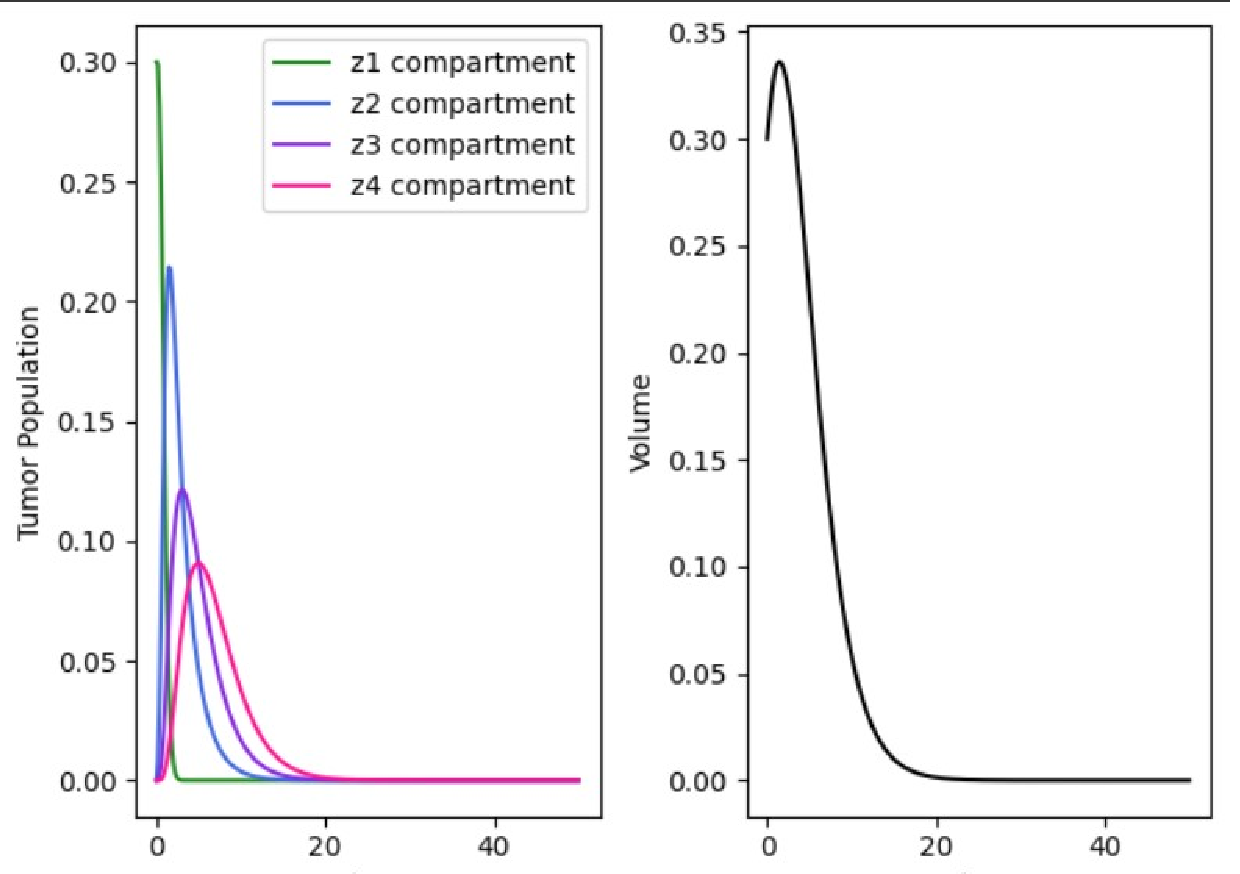
\includegraphics[width=\textwidth]{original_tumor_random_parameters.pdf}. % Better to make them pdfs than png or gif or jpeg
\end{center}
\caption{This graph shows our Simeoni graphs created with parameters: $\lambda_0=.5, \lambda_1=.2, \psi=.5, k_1 = .4, k_2=.5, c=t, V_0 = .3$. These parameters were arbitrarily chosen, but show that tumors could be treated.}
\label{fig:1}
\end{figure}

Various techniques and methods have been historically employed to tackle the challenge of modeling tumor growth and decay. Prior studies have explored models such as Mendelsohn, Exponential, Linear, Logistic, and Bertalanffy, among others \cite{Murphy_Hope_2016}. Each of these models brings a unique perspective to the understanding of tumor dynamics. While Simeoni is one of the models in this repertoire, we recognize the importance of critically evaluating its suitability and effectiveness compared to alternative models.

The intricacies of the Simeoni model motivate a fundamental question: is the existing Simeoni model the best model for the decay and growth of tumor cells, or are there adjustments that could enhance its precision in describing this phenomenon? A study conducted in 2020 showed that compared to other existing tumor growth functions, such as the generalized logistic, Gompertz, and Von Bertalanffny tumor growth functions, the Simeoni tumor growth function describes experimental data best, with minimal AIC, AICc, and BIC values\cite{Koziol_Falls_Schnitzer_2020}  The weights that were found also underscore the preference for the Simeoni tumor growth function.

As such, we did not alter the Simeoni tumor growth function or the number of peripheral compartments. Instead, we decided to focus on the Simeoni model as it is. We first examined its equilibria and the stability of the system at each equilibrium. An initial look at the system of ODEs shows that there is an equilibrium when each $Z_i = 0$. This occurs at $t=0$ an , so we have $Z_1(0) = Z_2(0) = Z_3(0) = Z_4(0)$. To confirm that this was the only equilibrium, we created a \verb!numpy! array representing the system, and calculated the null space. This proved that for the original Simeoni model, there is one equilibrium at the origin. To examine the stability of the origin, we calculated the eigenvalues of the matrix representing the model, corresponding to each $Z_i = 0$. If we use $k_1 = 0.4$, $k_2 = 0.5$, $c(t) = 0.5$, and $TGF(t) \approx 0.075$, our eigenvalues are $\lambda_1 = -0.5$, $\lambda_2 = -0.5$, $\lambda_3 = -0.5$, and $\lambda_4 \approx -0.125$. Since these values are all less than zero, we found that the origin is a stable equilibrium.

Next, we examined the effects of variation of the model’s parameters, such as $k_1$, $k_2$, $\lambda_0$, $\lambda_1$, $psi$, and $V_0$ on tumor population. We wanted to determine if by altering the parameters, we could significantly decrease the growth of tumor cells or even completely annihilate all tumor cells. We used \verb!python! to define our system of ODEs (1.1) and \verb!matplotlib! to visualize the graphs. We solved our IVP with Scipy \verb!solve_ivp! and then plotted these solutions to observe each compartment's behavior. We explored various parameter combinations and found a set of parameter values that model the tumor growth most realistically and similarly to existing research \cite{Koziol_Falls_Schnitzer_2020}. See figure \ref{fig:2} for a visual representation of that model. 

\begin{figure}[h]
\begin{center} %Put your images in a figure like this
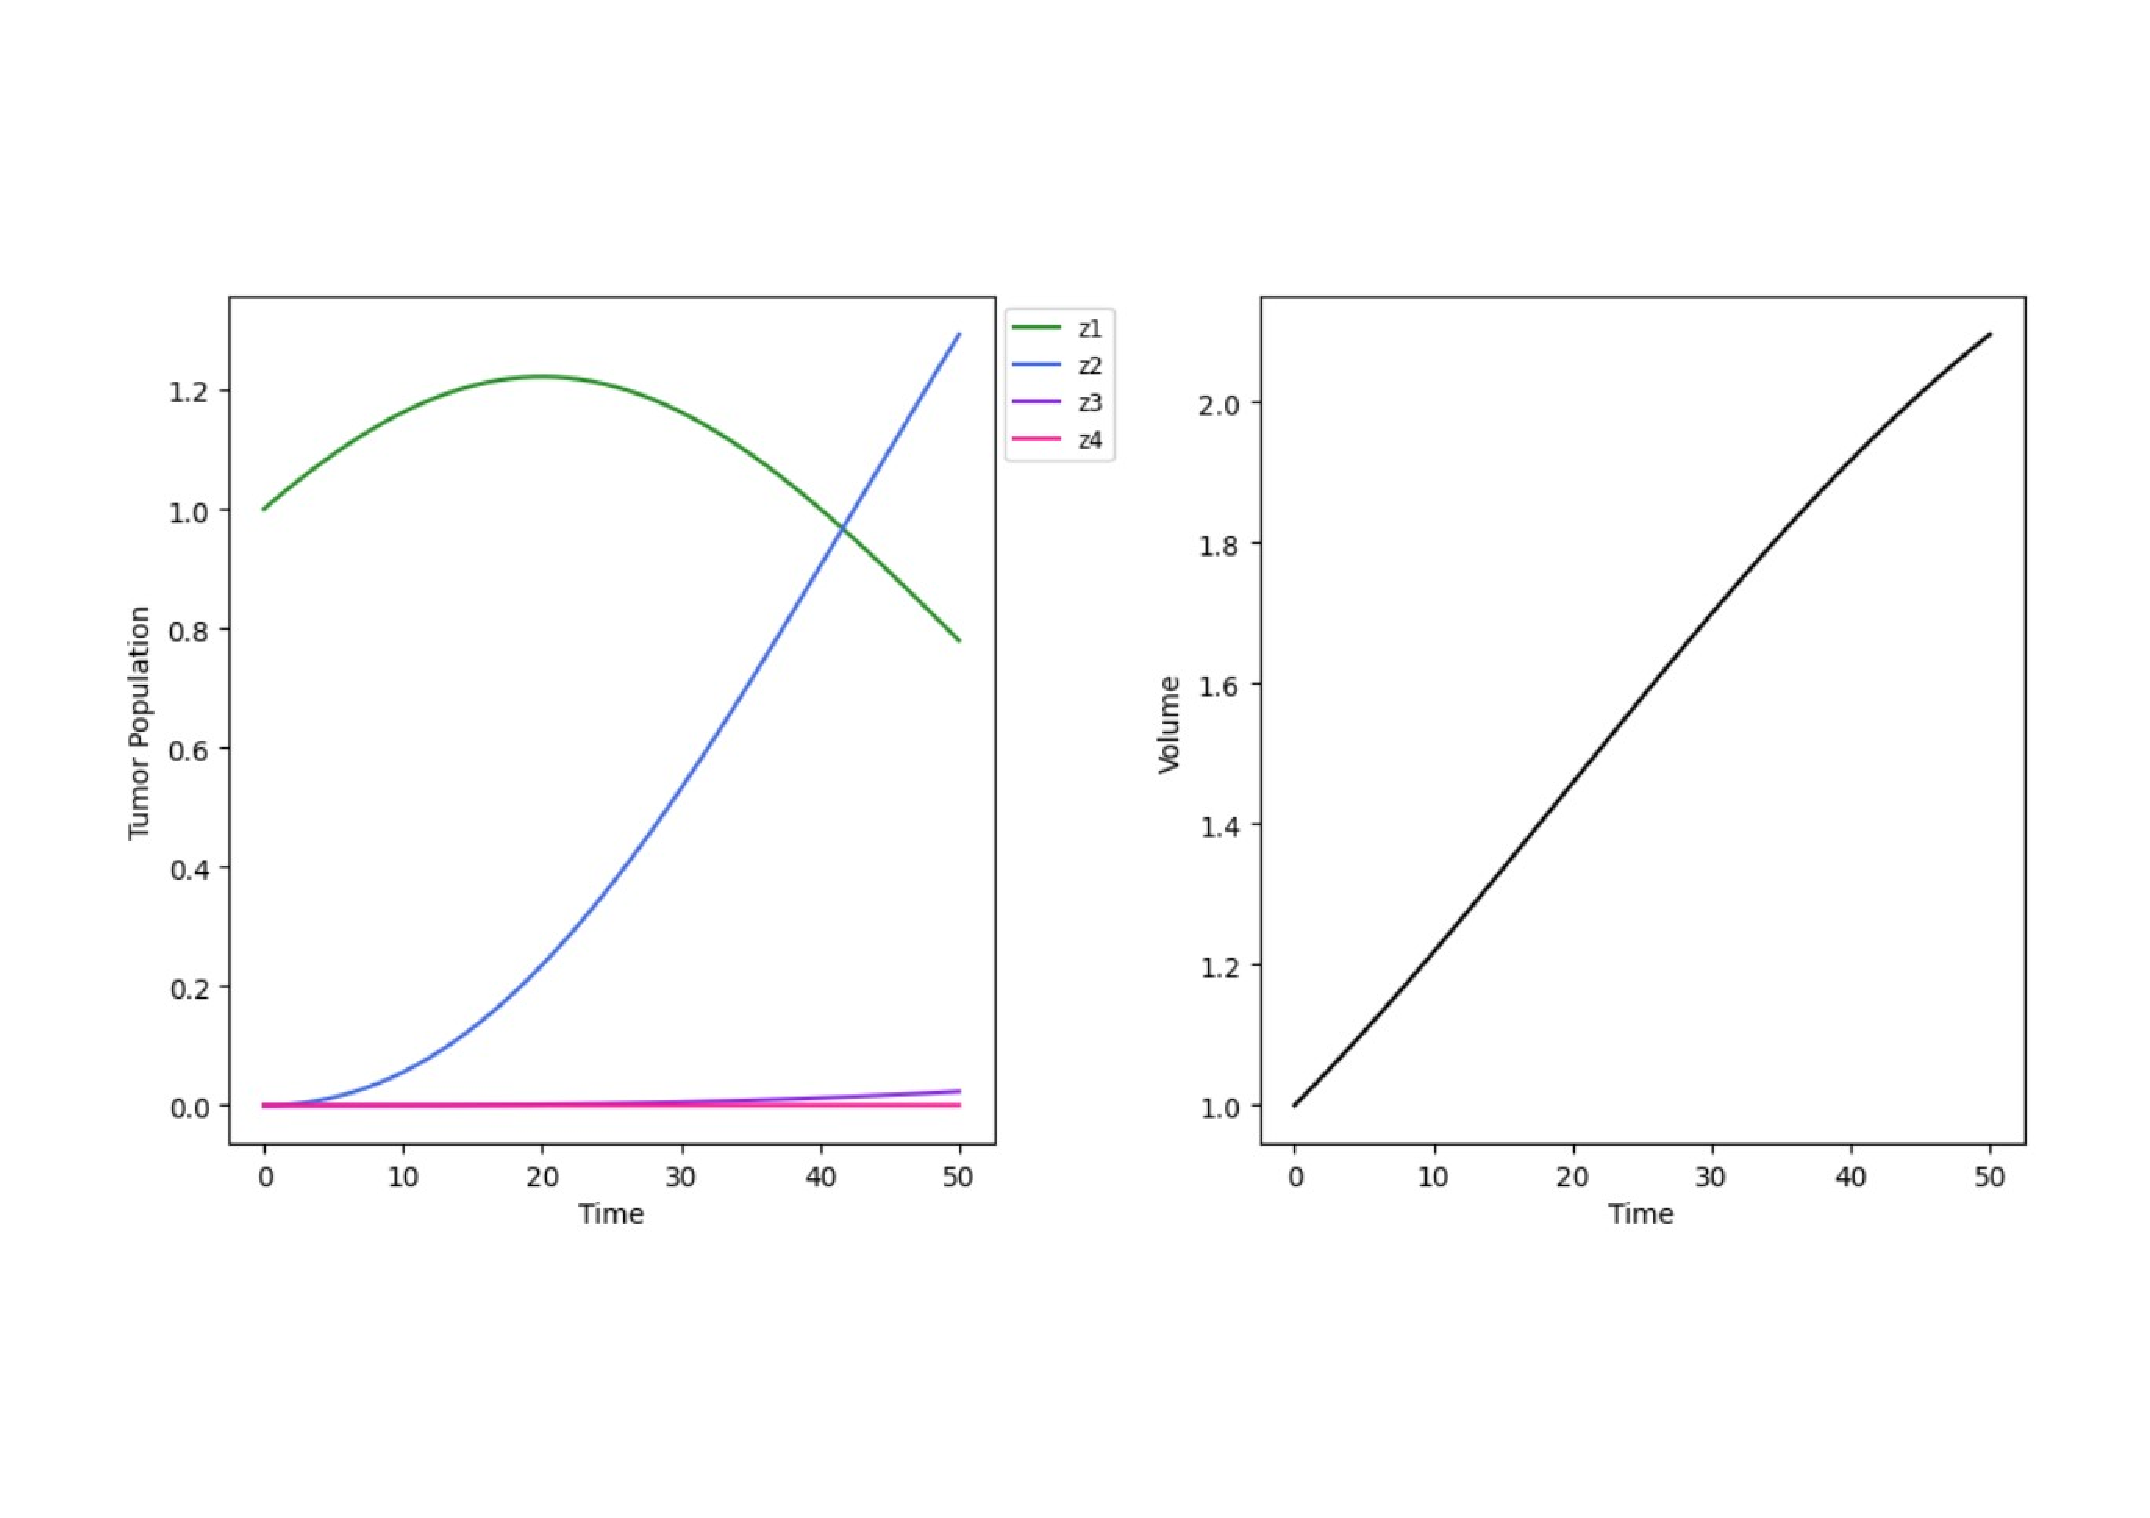
\includegraphics[width=\textwidth]{parameters_like_paper.pdf}. % Better to make them pdfs than png or gif or jpeg
\end{center}
\caption{Realistic valued model, with parameters: $\lambda_0=0.02, \lambda_1=0.001, \psi=-2, c=t, k_1=0.001, k_2=0.001, V_0=1$. This model is realistic because it models treatment of the tumor, with decreased Z1 values.}
\label{fig:2}
\end{figure}


\begin{remark}
\label{Remark 1.2}
    The graph in Figure \ref{fig:5} shows that the overall tumor volume continues to increase, although the rate slightly changes during the plotted time frame, which can be attributed to the delayed effect of treatment. Tumor cells are indeed moving from $Z_1$ to $Z_2$ and some have continued to $Z_3$. Given more time, we expect to see tumors continuously moving to $Z_3$ and $Z_4$ and eventually dying off. Depending on the specific treatment values as well as the stage of cancer, we can expect the tumor volume to continue to increase at slower rates or even begin decreasing. In the latter case, the effect of the birth of new tumor cells according to the tumor growth function is suppressed by the killing constants.
\end{remark}

Allowing for $c(t)$, the concentration of the treatment agent in $Z_1$, to equal zero at all values of t gives us tumor growth in the absence of any treatment. This is modeled in Figure \ref{fig:3} to visualize untreated tumor growth over time. Compare with Figure \ref{fig:2}, which has the same given parameters. It is worth noting that we do observe what we would expect to observe. Under the same given parameters, there is higher tumor volume over time in the absence of treatment than there is under treatment.

Just as no model can claim absolute perfection in its descriptive capabilities, the Simeoni model has certain limitations as well. Tumor growth in real-life scenarios, like any other real data, is characterized by noise and uncertainty. There is always a degree of randomness that the differential equations of the Simeoni model do not capture. Moreover, the model’s relevance and accuracy are examined through data from animal experimentation rather than human experimentation; this introduces another level of uncertainty. In addition, while the Simeoni tumor growth function captures experimental animal data best as compared with other growth functions, it is not the most biologically realistic growth law for application to humans \cite{Koziol_Falls_Schnitzer_2020}. With continuous research and comparison with other models and datasets, the Simeoni model and its tumor growth function can be further adapted or serve as a baseline for an eventual optimized model that can be realistically applied to humans. A 2020 study \cite{Koziol_Falls_Schnitzer_2020} found that the optimal number of peripheral compartments within the model remains uncertain concerning the goodness of fit. As the number of peripheral compartments is arbitrary yet also a crucial factor in modeling the results of treatment, potential weaknesses in this uncertainty should be acknowledged. As of this writing, there is no consensus as to which model best characterizes tumor growth. Despite its weaknesses, the Simeoni model remains one of the most robust tumor growth models in the field. 

\begin{figure}[h]
\begin{center} %Put your images in a figure like this
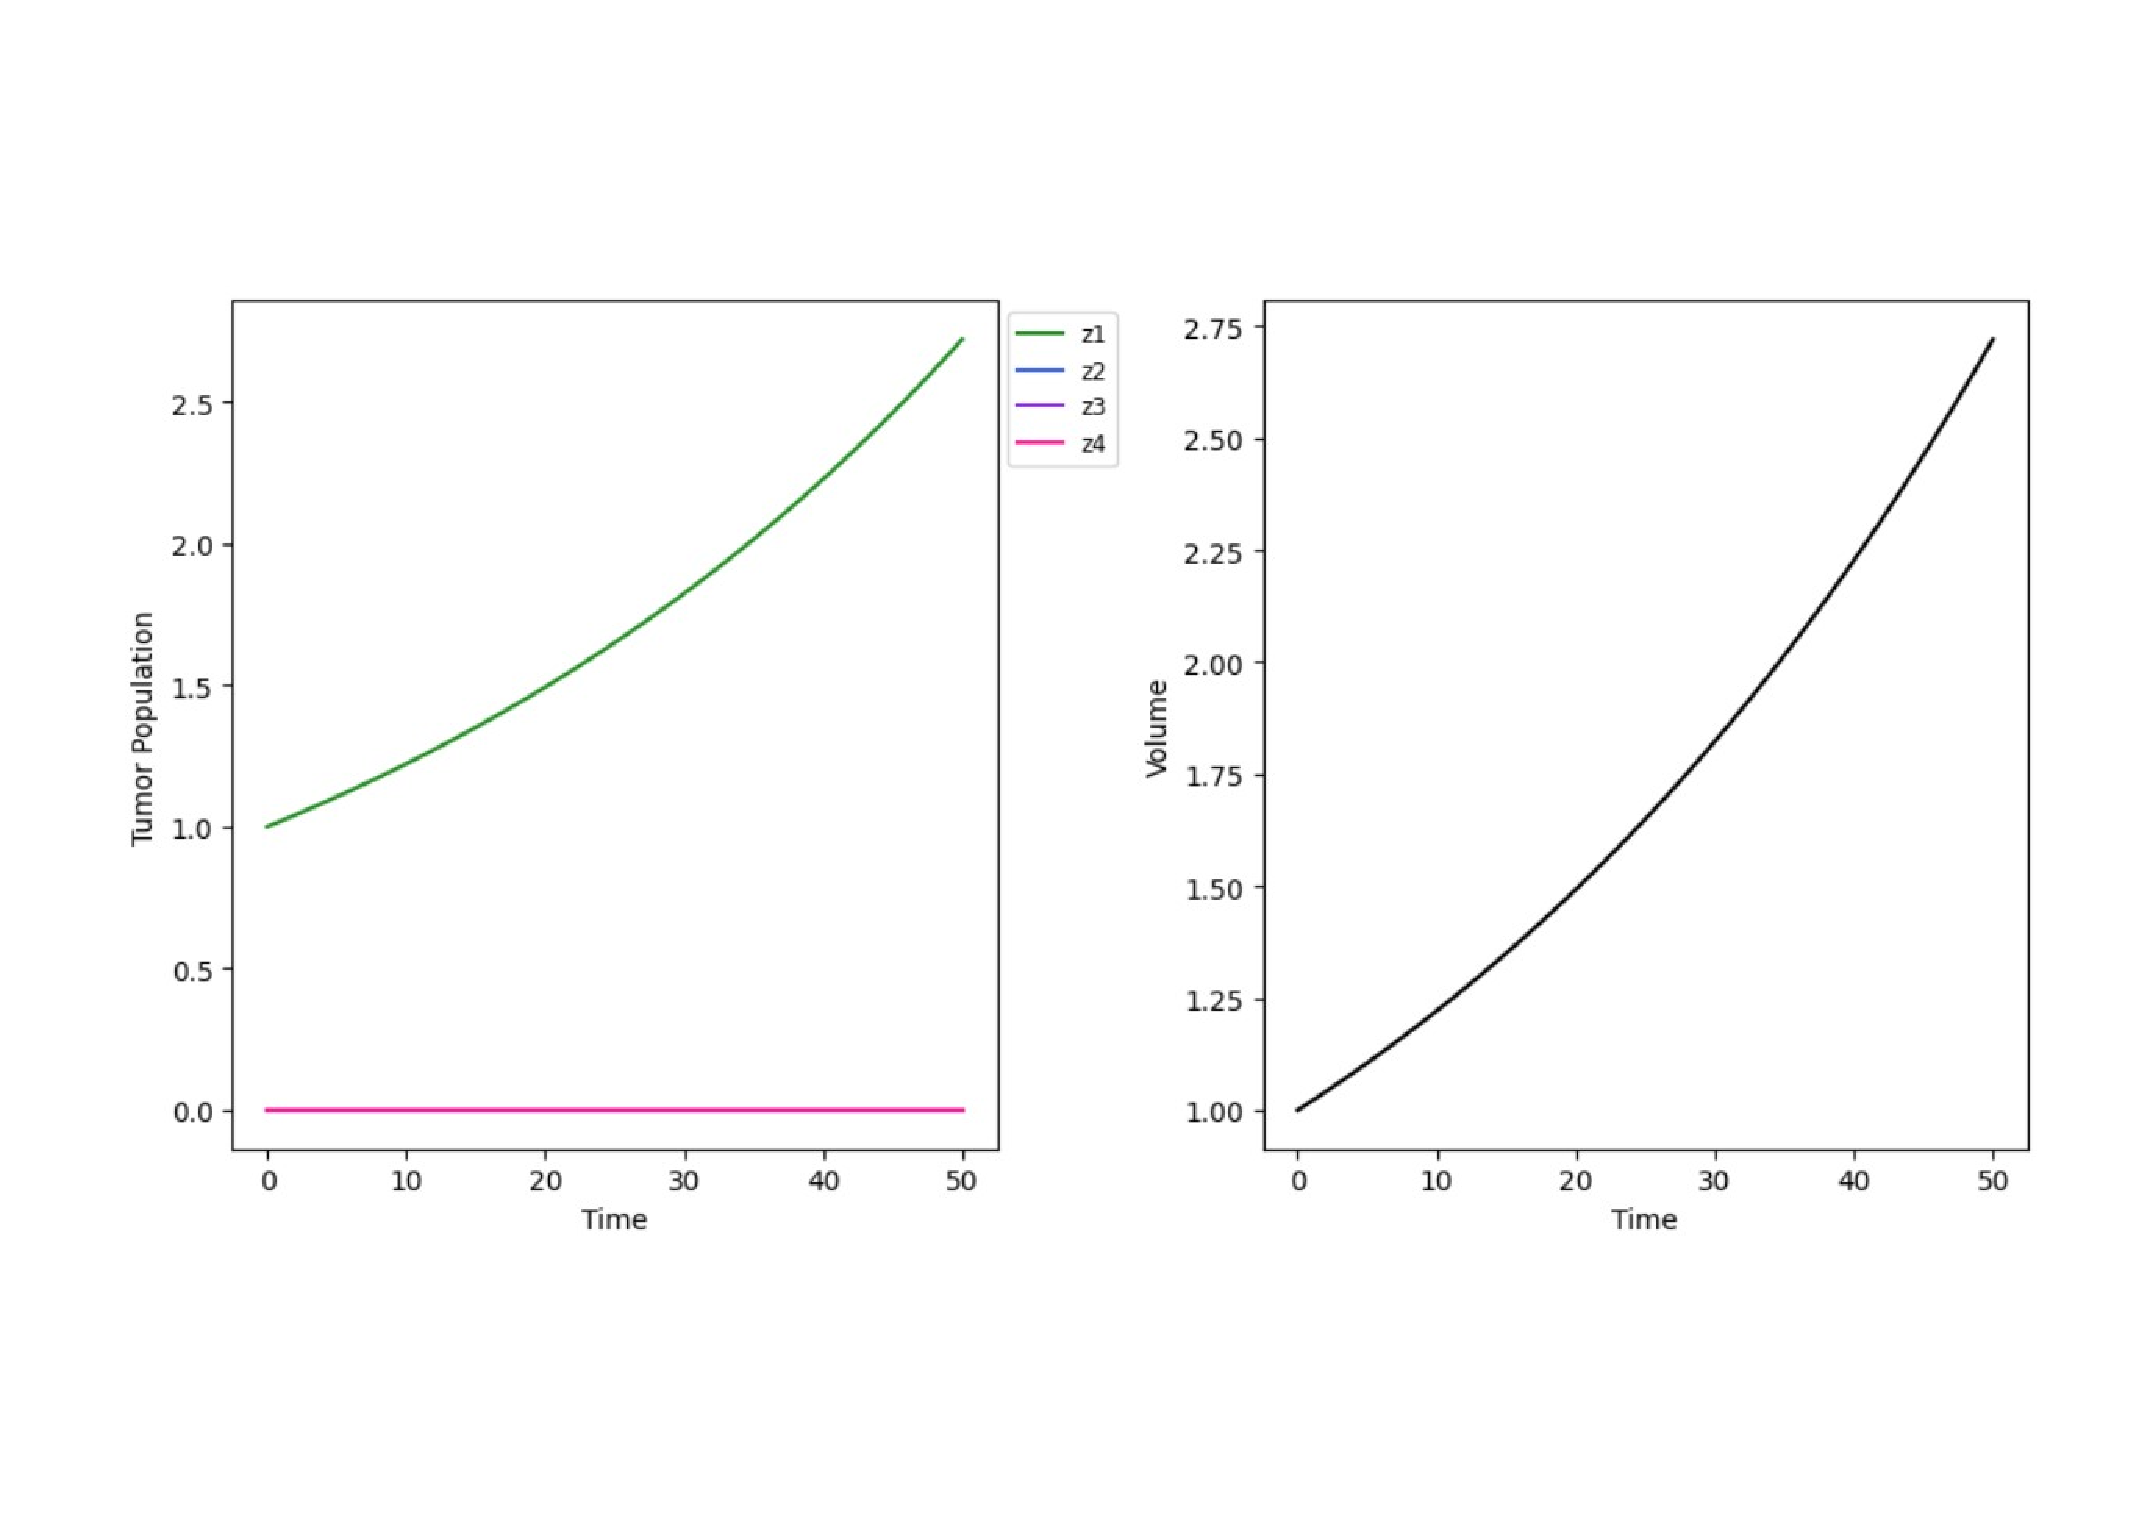
\includegraphics[width=\textwidth]{parameters_like_paper_no_treatment.pdf}. % Better to make them pdfs than png or gif or jpeg
\end{center}
\caption{Realistic valued model, with no treatment}
\label{fig:3}
\end{figure}

\begin{figure}[h]
\begin{center} %Put your images in a figure like this
\includegraphics[width=\textwidth]{compartments.pdf}. % Better to make them pdfs than png or gif or jpeg
\caption{This figure is from "Different ODE models of tumor growth can deliver similar results"\cite{Koziol_Falls_Schnitzer_2020}. It shows the tumor growth happening in Z1 and the delayed growth from tumor treatment. The fact that there are four compartments in the model ($Z_1$, $Z_2$, $Z_3$, and $Z_4$) is arbitrary, and models different stages of . Our model fits this figure's depiction of the stages of tumor growth.}
\end{center}
\label{fig:4}
\end{figure}



Figure \ref{fig:1} and Figure \ref{fig:5} illustrate the rapid decrease of tumor volume upon increasing the values of the constant parameters. With specific parameter values as outlined in the respective captions, we find that we can not only slow tumor growth rate but also completely eradicate all tumors. As seen in Figure \ref{fig:1}, all tumors are essentially gone within 20 days.

\begin{figure}[h]
\begin{center} %Put your images in a figure like this
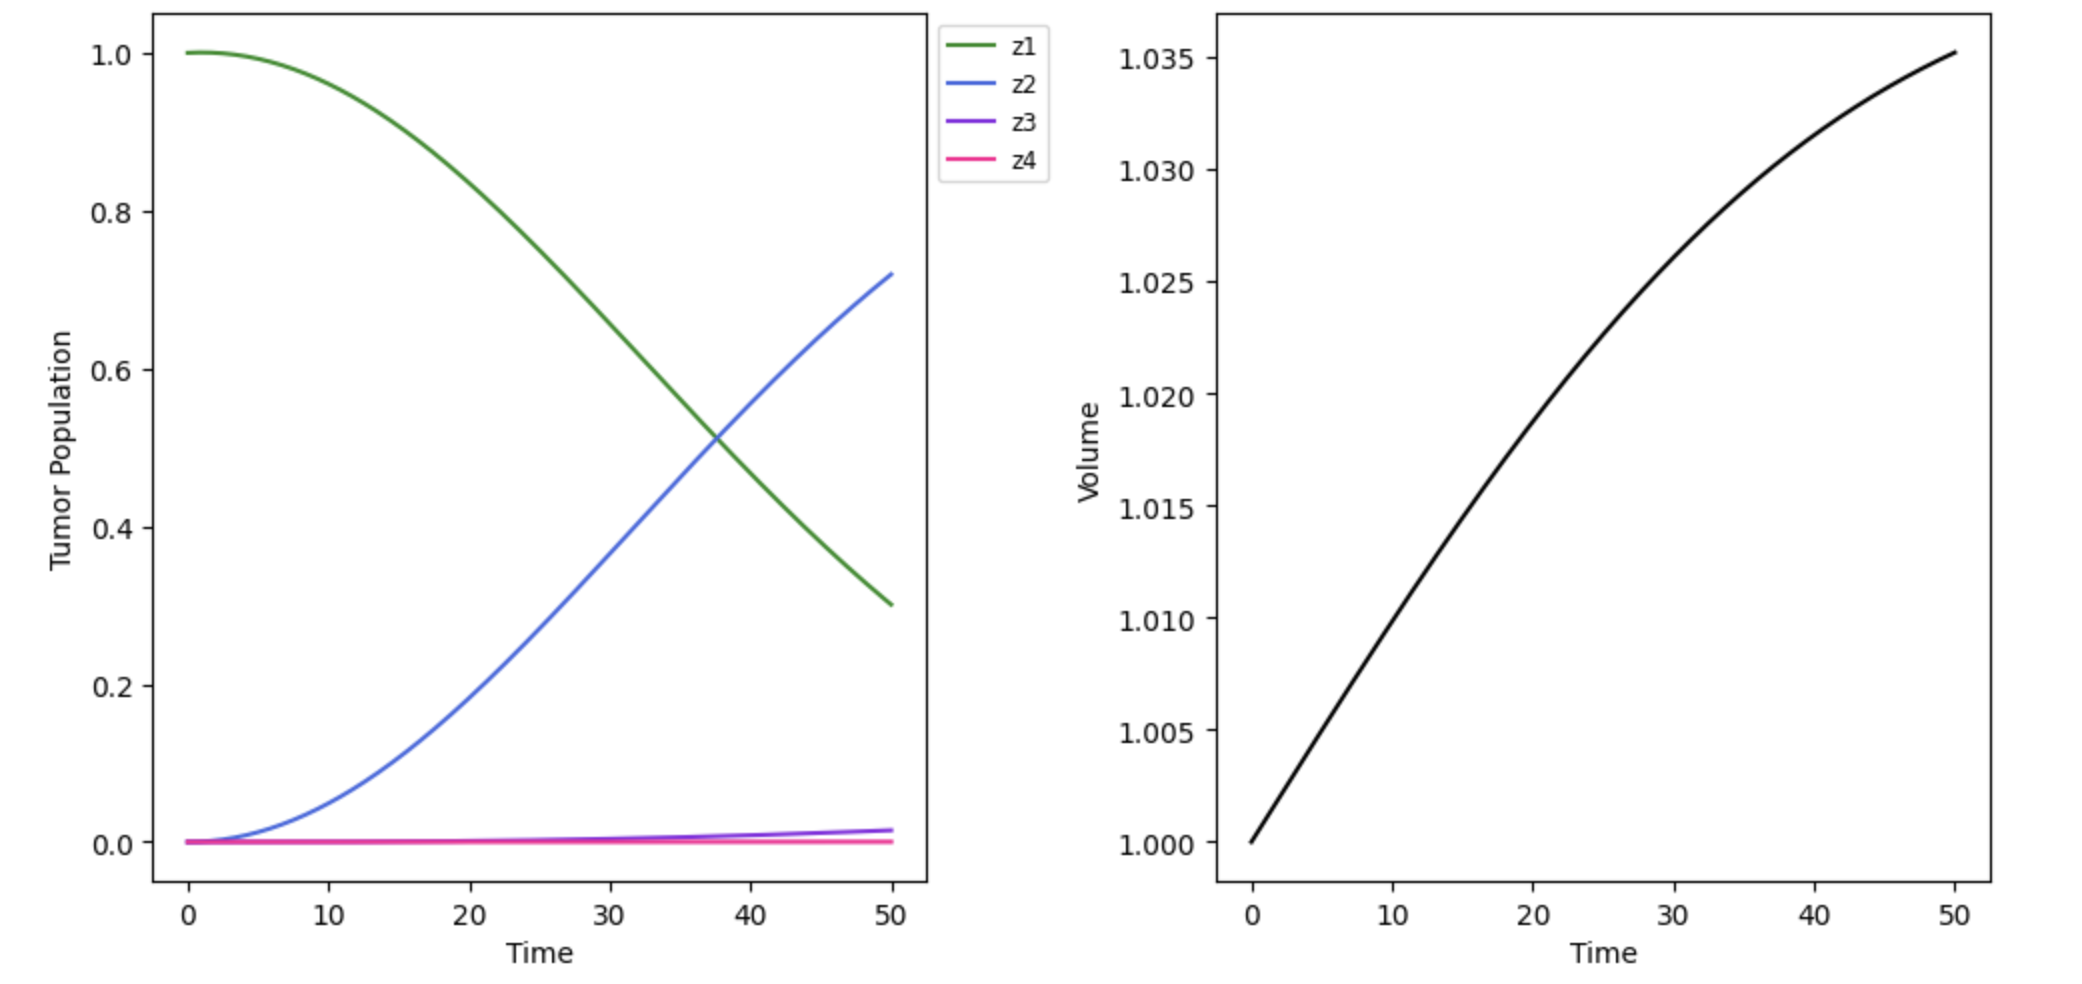
\includegraphics[width=\textwidth]{altered.png}. % Better to make them pdfs than png or gif or jpeg
\end{center}
\caption{Our altered-parameters-valued model with parameters $\lambda_0=0.02, \lambda_1=0.001, \psi=2, k_1 = 0.001, k_2=0.001, V_0 = 1$}
\label{fig:5}
\end{figure}



%% Third Section
\section{Results}
%Talk about how if we can build a cancer treatment to model this it would be great!
Concerning the model’s stability, we found that it is based on the existence of one stable equilibrium at the origin. This equilibrium satisfies the definition of a uniformly stable system and is crucial for maintaining the system's stability and consistent behavior. 

After conducting deep parameter tuning, we can affirm that the Simeoni model can realistically reflect the chemotherapeutic and immunotherapeutic treatment on tumor growth. In the absence of such treatment agents, tumor growth is increased.

We also found that when each constant parameter is increased relative to the constant parameter setting of the realistic model (see Figure \ref{fig:2}), tumor growth increases at a slower rate. With parameter values high enough, the overall tumor volume even eventually returns to zero, signifying a state void of any remaining tumor cells. This potentially has very significant implications: if the constant parameters can be realistically and ethically manipulated to attain the values as in our altered model, the efficacy of the same levels of chemotherapeutic and immunotherapeutic agents can be greatly increased. Nonetheless, these findings suggest that even minimally increasing the values of the constant parameters can have positive effects on slowing tumor growth.

Figure \ref{fig:1} and Figure \ref{fig:4} illustrate the rapid decrease of tumor volume upon increasing the values of the constant parameters. With specific parameter values as outlined in the respective captions, we find that we can not only slow tumor growth rate but also completely eradicate all tumors. As seen in Figure \ref{fig:1}, all tumors are essentially gone within 20 days.



Again, it is important to explore the feasibility of directly manipulating these parameters in real-world scenarios to determine the optimal, realistic combination for achieving the most effective cancer treatment.  


%%Fourth Section
\section{Analysis/Conclusions}
The techniques and methods employed in our modeling endeavors were crucial in gaining insights into the dynamics of cancer progression. We chose to model treated tumors within the body, which we feel the Simeoni model does well. Through our analysis, we observed both successes and challenges in capturing the intricacies of the chosen phenomenon. The appropriateness of the methods became evident as they allowed us to simulate and understand the growth patterns of cancerous tumors. 

However, we acknowledge that the modeling process presented its own set of complexities, and while our group made significant strides, there remains room for improvement. Given more time, we would like to do more research on tumors to be more informed and to be able to modify the model by adding new variables and functions as well as find a better explanation of the types of constants that model tumor growth appropriately. In addition, we would like to explore and dissect the Simeoni model further by altering the c(t) function. Findings from these particular alterations can lend insight into optimal amounts of chemotherapeutic and immunotherapeutic agent concentrations at different times. Experimenting with different initial values of Z1 can lend valuable insight into the efficacy of treatment at earlier vs later and slower vs rapid onset stages of cancer.

In the event of a successful modification of the Simeoni Model, our findings could have far-reaching implications for cancer treatment strategies. The ability to predict and understand tumor growth patterns more accurately could inform personalized treatment plans and optimize the allocation of resources in healthcare. Our research emphasizes the significance of dynamic modeling in the context of cancer research and the potential impact on treatment efficiency and patient outcomes. 

Our goal was to educate ourselves and any potential audience of an example of a system of ODEs that appropriately models how a tumor grows and depletes as it is treated. Though models are never perfect, we believe we can learn more about tumors and how to properly treat them by observing what different parameters are most effective in stopping tumor growth. The lessons learned from our research methodology can also be applied to other areas of scientific inquiry, providing a framework for tackling complex biological processes. We encourage others to appreciate the interdisciplinary nature of modeling and its potential to drive advancements in healthcare and beyond.


% \begin{figure}[h]
% \begin{center} %Put your images in a figure like this
% \includegraphics[width=\textwidth]{Myfig.pdf}. % Better to make them pdfs than png or gif or jpeg
% \end{center}
% \label{fig:MatrixError}
% \end{figure}





%%%%%%%%%%%%%%%%%%%%%%%%%%%%%%%%%%%%%
%% Bibliography below
%%%%%%%%%%%%%%%%%%%%%%%%%%%%%%%%%%%%%
\FloatBarrier % Keep the figures from being put after the bibliography
\newpage
%% If using bibtex, leave this uncommented
\bibliographystyle{plain}
\bibliography{refs}{} %if using bibtex, call your bibtex file refs.bib

%% If not using bibtex, comment out the previous two lines and uncomment those below
%%\begin{thebibliography}{99}
   %% \bibitem{article}
     %%   Koziol, J.A., Falls, T.J. & Schnitzer, J.E. Different ODE models of tumor growth can deliver similar  results. BMC Cancer 20, 226 (2020). https://doi.org/10.1186/s12885-020-6703-0
    %%\bibitem{article}
     %%   Murphy, H., Jaafari, H. & Dobrovolny, H.M. Differences in predictions of ODE models of tumor growth: a cautionary example. BMC Cancer 16, 163 (2016). https://doi.org/10.1186/s12885-016-2164-x
     
%%\end{thebibliography}

\end{document}